% Siconos is a program dedicated to modeling, simulation and control
% of non smooth dynamical systems.
%
% Copyright 2016 INRIA.
%
% Licensed under the Apache License, Version 2.0 (the "License");
% you may not use this file except in compliance with the License.
% You may obtain a copy of the License at
%
% http://www.apache.org/licenses/LICENSE-2.0
%
% Unless required by applicable law or agreed to in writing, software
% distributed under the License is distributed on an "AS IS" BASIS,
% WITHOUT WARRANTIES OR CONDITIONS OF ANY KIND, either express or implied.
% See the License for the specific language governing permissions and
% limitations under the License.
%
\documentclass[10pt]{article}



\usepackage{a4wide}
\usepackage{amsmath}
\usepackage{amssymb}
\usepackage{minitoc}
%\usepackage{glosstex}
\usepackage{colortbl}
\usepackage{hhline}
\usepackage{longtable}

\def\glossaryname{Glossary of Notation}



\usepackage{color}
\usepackage{graphicx,epsfig}
\graphicspath{{figure/}}
\usepackage[T1]{fontenc}
\usepackage{rotating}

\usepackage{algorithmic}
\usepackage{algorithm}
%\usepackage{ntheorem}
\usepackage{natbib}

\renewcommand{\algorithmiccomment}[1]{//#1}

%\renewcommand{\baselinestretch}{2.0}
\setcounter{tocdepth}{2}     % Dans la table des matieres
\setcounter{secnumdepth}{3}  % Avec un numero.



%\newtheorem{definition}{Definition}
%\newtheorem{lemma}{Lemma}
%\newtheorem{claim}{Claim}
%\newtheorem{remark}{Remark}
%\newtheorem{assumption}{Assumption}
%\newtheorem{example}{Example}
%\newtheorem{conjecture}{Conjecture}
%\newtheorem{corollary}{Corollary}
%\newtheorem{OP}{OP}
%\newtheorem{problem}{Problem}
%\newtheorem{theorem}{Theorem}


\newcommand{\CC}{\mbox{\rm $~\vrule height6.6pt width0.5pt depth0.25pt\!\!$C}}
\newcommand{\ZZ}{\mbox{\rm \lower0.3pt\hbox{$\angle\!\!\!$}Z}}
\newcommand{\RR}{\mbox{\rm $I\!\!R$}}
\newcommand{\NN}{\mbox{\rm $I\!\!N$}}

\newcommand{\Frac}[2]{\displaystyle \frac{#1}{#2}}

\newcommand{\DP}[2]{\displaystyle \frac{\partial {#1}}{\partial {#2}}}


\newcommand{\ie}{i.e.}
\newcommand{\eg}{e.g.}
\newcommand{\cf}{c.f.}
\newcommand{\putidx}[1]{\index{#1}\textit{#1}}

\def\Er{{\rm I\! R}}
\def\En{{\rm I\! N}} 
\def\Ec{{\rm I\! C}}
 






%----------------------------------------------------------------------
%                  Modification des subsubsections
%----------------------------------------------------------------------
\makeatletter
\renewcommand\thesubsubsection{\thesubsection.\@alph\c@subsubsection}
\makeatother

%----------------------------------------------------------------------
%             Redaction note environnement
%----------------------------------------------------------------------
\makeatletter
%\theoremheaderfont{\scshape}
%\theoremstyle{marginbreak}
%\theorembodyfont{\upshape}
%\newtheorem{rque}{\bf Remarque}[chapter]
%\newtheorem{rque1}{\bf \fsc{Remarque}}[chapter] !!! \fsc est une commande french
%\newtheorem{ndr1}{\textbf{\textsc{Redaction note}}}[section]

\newenvironment{ndr}%
{%
\tt
%\centerline{---oOo---}
\noindent\begin{ndr1}%
}%
{%
\begin{flushright}%
%\vspace{-1.5em}\ding{111}
\end{flushright}%
\end{ndr1}%
%\centerline{---oOo---}
}

\makeatother

%----------------------------------------------------------------------
%             Redaction note environnement V.ACARY
%----------------------------------------------------------------------
\makeatletter
%\theoremheaderfont{\scshape}
%\theoremstyle{marginbreak}
%\theorembodyfont{\upshape}
%\newtheorem{rque}{\bf Remarque}[chapter]
%\newtheorem{rque1}{\bf \fsc{Remarque}}[chapter] !!! \fsc est une commande french
%\newtheorem{ndr1va}{\textbf{\textsc{Redaction note V. ACARY}}}[section]

\newenvironment{ndrva}%
{%
\tt
%\centerline{---oOo---}
\noindent\begin{ndr1va}%
}%
{%
\begin{flushright}%
%\vspace{-1.5em}\ding{111}
\end{flushright}%
\end{ndr1va}%
%\centerline{---oOo---}
}

\makeatother




%%% Local Variables: 
%%% mode: latex
%%% TeX-master: "report"
%%% End: 

\usepackage{psfrag}
\usepackage{fancyhdr}
\usepackage{subfigure}
%\renewcommand{\baselinestretch}{1.2}
\textheight 23cm
\textwidth 16cm
\topmargin 0cm
%\evensidemargin 0cm
\oddsidemargin 0cm
\evensidemargin 0cm
\usepackage{layout}
\usepackage{mathpple}
\makeatletter
\renewcommand\bibsection{\paragraph{References
     \@mkboth{\MakeUppercase{\bibname}}{\MakeUppercase{\bibname}}}}
\makeatother
%% style des entetes et des pieds de page
\fancyhf{} % nettoie le entetes et les pieds
\fancyhead[L]{Template 6 : Electrical oscillator with 4 diodes bridge full-wave rectifier - Pascal Denoyelle}
%\fancyhead[C]{}%
\fancyhead[R]{\thepage}
%\fancyfoot[L]{\resizebox{!}{0.7cm}{\includegraphics[clip]{logoesm2.eps}}}%
\fancyfoot[C]{}%
%\fancyfoot[C]{}%
%\fancyfoot[R]{\resizebox{!}{0.7cm}{\includegraphics[clip]{logo_cnrs_amoi.ps}}}%
%\addtolength{\textheight}{2cm}
%\addtolength{\textwidth}{2cm}
%\pagestyle{empty}
%\renewcommand{\baselinestretch}{2.0}
\begin{document}
%\layout
\thispagestyle{empty}
\title{WP2 Template 6 \\Simulation of an electrical oscillator supplying a resistor\\
through a 4 diodes bridge full-wave rectifier}
\author{Pascal Denoyelle}

\date{Version 1.0 \\
 September 23 , 2005}
\maketitle


\pagestyle{fancy}

\section{Description of the physical problem : electrical oscillator with 4 diodes bridge full-wave rectifier}
In this sample, a LC oscillator initialized with a given voltage across the capacitor and a null current through
the inductor provides the energy
to a load resistance through a full-wave rectifier consisting of a 4 ideal diodes bridge (see fig. \ref{fig-DiodeBridge}).

\begin{figure}[hp]
\centerline{
  \scalebox{0.75}{
     \input{Bridge.pstex_t}
  }
}
\caption{Electrical oscillator with 4 diodes bridge full-wave rectifier}
\label{fig-DiodeBridge}
\end{figure}

Both waves of the oscillating voltage across the LC are provided to the resistor with current flowing always in 
the same direction. The energy is dissipated in the resistor resulting in a damped oscillation.


\section{Definition of a general abstract class of NSDS : the linear time invariant complementarity system (LCS)}
\label{sec-def-NSDS}
This type of non-smooth dynamical system consists of :

\begin{itemize}
\item a time invariant linear dynamical system (the oscillator). The state variable of this system is denoted by $x$.
\item a non-smooth law describing the behaviour of each diode of the bridge as a complementarity condition between current and
reverse voltage (variables ($y,\lambda$) ). Depending on the diode position in the bridge, $y$ stands for the reverse voltage 
across the diode or for the diode current.
\item a linear time invariant relation between the state variable $x$ and the non-smooth law variables ($y,\lambda$)
\end{itemize}

\subsection{Dynamical system and Boundary conditions}
\underline{Remark :}
In a more general setting, the system's evolution would be described by a DAE :
\[
G \cdot x' = A \cdot x + E \cdot u + b + r 
\]
with $G , A , E$ matrices constant over time (time invariant system), $u , b$ source terms functions of time and $r$,
a term coming from the non-smooth law variables : $r = B \cdot \lambda + a$ with $B , a$ constant over time.\\
We will consider here the case of an ordinary differential equation :
\[
x' = A \cdot x + E \cdot u + b + r 
\]
and an initial value problem for which the boundary conditions are $t_0 \in \mathbb{R} , x(t_0)= x_0$.

\subsection{Relation between constrained variables and state variables}
In the linear time invariant framework, the non-smooth law acts on the linear dynamical system evolution through the variable 
$r = B \cdot \lambda + a$. Reciprocally, the state variable $x$ acts on the non-smooth law through the relation
$y = C \cdot x + D \cdot \lambda + F \cdot u + e$ with $C , D , F , e$ constant over time.

\subsection{Definition of the Non Smooth Law between constrained variables}
It is a complementarity condition between y and $\lambda$ : $0 \leq y \, \perp \, \lambda \geq 0$. This corresponds
to the behaviour of the rectifying diodes, as described in \ref{Non Smooth laws}.
 
\section{The formalization of the electrical oscillator with 4 diodes bridge full-wave rectifier into the LCS}

The equations come from the following physical laws :
\begin{itemize}
\item the Kirchhoff current law (KCL) establishes that the sum of the currents arriving at a node is zero,
\item the Kirchhoff voltage law (KVL) establishes that the sum of the voltage drops in a loop is zero,
\item the branch constitutive equations define the relation between the current through a bipolar device
and the voltage across it
\end{itemize}
Refering to figure \ref{fig-DiodeBridge}, the Kirchhoff laws could be written as :
\[
\begin{array}{l}
v_L = v_C\\
v_L = v_{DF1} - v_{DR1}\\
v_{DF1} + v_R + v_{DR2} = 0\\
v_{DF2} + v_R + v_{DR1} = 0\\

i_C + i_L + i_{DF1} - i_{DR2} = 0\\
i_{DF1} + i_{DR1} = i_R\\
i_{DF2} + i_{DR2} = i_R\\
\end{array}
\]
while the branch constitutive equations for linear devices are :
\[
\begin{array}{l}
i_C = C v_C'\\
v_L = L i_L'\\
v_R = R i_R
\end{array}
\]
and last the "branch constitutive equation" of the ideal diodes that is no more an equation but instead
a complementarity condition :
\[ 
\begin{array}{l}
0 \leq i_{DF1} \, \perp \, -v_{DF1} \geq 0\\
0 \leq i_{DR1} \, \perp \, -v_{DR1} \geq 0\\
0 \leq i_{DF2} \, \perp \, -v_{DF2} \geq 0\\
0 \leq i_{DR2} \, \perp \, -v_{DR2} \geq 0
\end{array}
\]
This is illustrated on figure \ref{fig-diode-reg} where the left-hand sketch displays the ideal diode 
characteristic and the right-hand sketch displays the usual exponential characteristic as stated by
Shockley's law.

\begin{figure}[htp]
\begin{center}
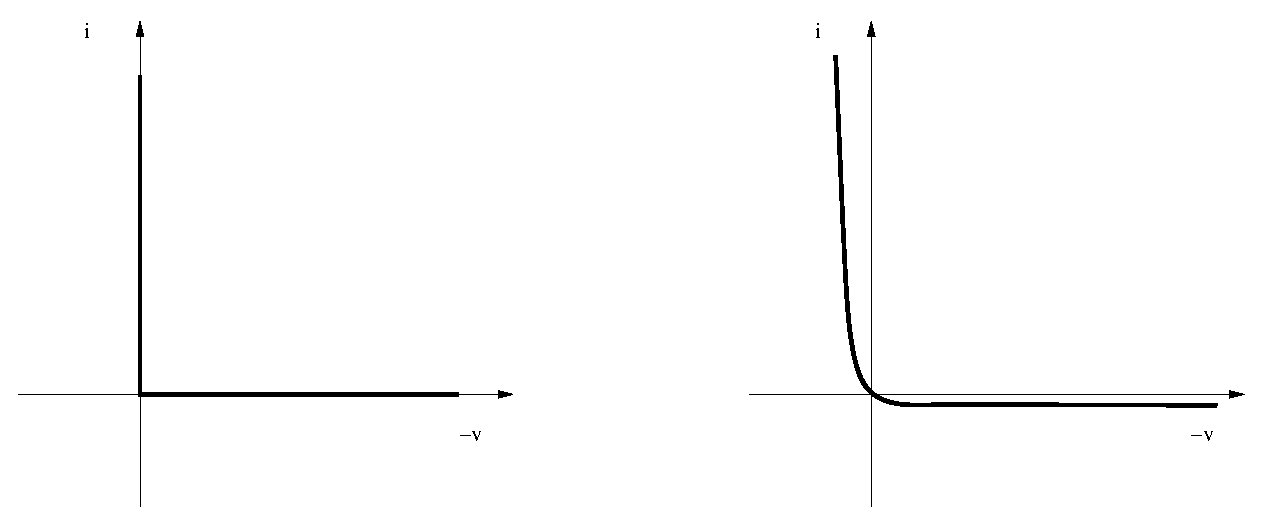
\includegraphics[width=12cm]{diode-caract.eps}
\end{center}
\caption{Non-smooth and smooth characteristics of a diode}
\label{fig-diode-reg}
\end{figure}


\subsection{Dynamical equation}
\label{sec-dyn-eq}
After rearranging the previous equations, we obtain :
\[ 
\left( \begin{array}{c}
v_L'\\
i_L'
\end{array} \right)
=
\left( \begin{array}{cc}
0 & \frac{-1}{C}\\
\frac{1}{L} & 0
\end{array} \right)
 \cdot
\left( \begin{array}{c}
v_L\\
i_L
\end{array} \right)
+
\left( \begin{array}{cccc}
0 & 0 & \frac{-1}{C} & \frac{1}{C}\\
0 & 0 & 0 & 0
\end{array} \right)
 \cdot 
\left( \begin{array}{c}
-v_{DR1}\\
-v_{DF2}\\
i_{DF1}\\
i_{DR2}
\end{array} \right)
\]
that fits in the frame of \ref{sec-def-NSDS} with
\[
x = 
\left( \begin{array}{c}
v_L\\
i_L
\end{array} \right)
\]
and 
\[
\lambda = 
\left( \begin{array}{c}
-v_{DR1}\\
-v_{DF2}\\
i_{DF1}\\
i_{DR2}
\end{array} \right)
\]



\subsection{Relations}
We recall that the $r = B \cdot \lambda + a$ equation is expressed with

\[
r =
\left( \begin{array}{cccc}
0 & 0 & \frac{-1}{C} & \frac{1}{C}\\
0 & 0 & 0 & 0
\end{array} \right)
 \cdot 
\left( \begin{array}{c}
-v_{DR1}\\
-v_{DF2}\\
i_{DF1}\\
i_{DR2}
\end{array} \right)
\]
from the dynamical equation (\ref{sec-dyn-eq}).\\
Rearranging the initial set of equations yields :
\[
\left( \begin{array}{c}
i_{DR1}\\
i_{DF2}\\
-v_{DF1}\\
-v_{DR2}
\end{array} \right)
 = 
\left( \begin{array}{cc}
0 & 0\\
0 & 0\\
-1 & 0\\
1 & 0
\end{array} \right)
 \cdot
\left( \begin{array}{c}
v_L\\
i_L
\end{array} \right)
+
\left( \begin{array}{cccc}
\frac{1}{R} & \frac{1}{R} & -1 & 0\\
\frac{1}{R} & \frac{1}{R} & 0 & -1\\
1 & 0 & 0 & 0\\
0 & 1 & 0 & 0
\end{array} \right)
 \cdot
\left( \begin{array}{c}
-v_{DR1}\\
-v_{DF2}\\
i_{DF1}\\
i_{DR2}
\end{array} \right)
\]
as the second equation of the linear time invariant relation with 
\[
y = 
\left( \begin{array}{c}
i_{DR1}\\
i_{DF2}\\
-v_{DF1}\\
-v_{DR2}
\end{array} \right)
\]


\subsection{Non Smooth laws}
\label{Non Smooth laws}
There is just the complementarity condition resulting from the ideal diode characteristic :

\[ 
\begin{array}{l}
0 \leq -v_{DR1} \, \perp \, i_{DR1} \geq 0\\
0 \leq -v_{DF2} \, \perp \, i_{DF2} \geq 0\\
0 \leq i_{DF1} \, \perp \, -v_{DF1} \geq 0\\
0 \leq i_{DR2} \, \perp \, -v_{DR2} \geq 0
\end{array}
\]



\section{Description of the numerical simulation: the Moreau's time-stepping scheme}
\subsection{Time discretization of the dynamical system}
The integration of the ODE over a time step $[t_i,t_{i+1}]$ of length $h$ is :

\[
\int_{t_i}^{t_{i+1}}x'\,dt = \int_{t_i}^{t_{i+1}} A \cdot x\,dt + \int_{t_i}^{t_{i+1}}(E \cdot u + b) dt + \int_{t_i}^{t_{i+1}}r\,dt   
\]
The left-hand term is $x(t_{i+1})-x(t_i)$. \\
Right-hand terms are approximated this way :
\begin{itemize}
\item $\int_{t_i}^{t_{i+1}} A \cdot x\,dt$ is approximated using a $\theta$-method
\[
\int_{t_i}^{t_{i+1}} A \cdot x\,dt \approx h \theta (A \cdot x(t_{i+1})) + h (1-\theta) (A \cdot x(t_{i}))
\]

\item since the second integral comes from independent sources, it can be evaluated with whatever quadrature method, for
instance a $\theta$-method 
\[
\int_{t_i}^{t_{i+1}}(E \cdot u + b) dt \approx h \theta (E \cdot u(t_{i+1}) + b(t_{i+1})) + 
                                                              h (1-\theta) (E \cdot u(t_{i}) + b(t_{i}))
\]

\item the third integral is approximated like in an implicit Euler integration
\[
\int_{t_i}^{t_{i+1}}r\,dt \approx h r(t_{i+1})
\]
\end{itemize}
By replacing the accurate solution $x(t_i)$ by the approximated value $x_i$, we get :
\[
x_{i+1}-x_i = h \theta (A \cdot x_{i+1}) + h (1-\theta) (A \cdot x_{i}) + 
              h \theta (E \cdot u(t_{i+1}) + b(t_{i+1})) + h (1-\theta) (E \cdot u(t_{i}) + b(t_{i})) + h r_{i+1}
\]
Assuming that $I - h \theta A$ is invertible, matrix $W$ is defined as $(I - h \theta A)^{-1}$. We get then :
\[
x_{i+1} = W(I + h (1-\theta) A) \cdot x_{i} + 
            W (h \theta (E \cdot u(t_{i+1}) + b(t_{i+1})) + h (1-\theta) (E \cdot u(t_{i}) + b(t_{i}))) + h W r_{i+1}
\]
An intermediate variable $x_{free}$ related to the smooth part of the system is defined as :
\[
x_{free} = W(I + h (1-\theta) A) \cdot x_{i} + 
           W (h \theta (E \cdot u(t_{i+1}) + b(t_{i+1})) + h (1-\theta) (E \cdot u(t_{i}) + b(t_{i})))
\]
Thus the calculus of $x_{i+1}$ becomes :
\[
x_{i+1} = x_{free} + h W r_{i+1}
\]

\subsection{Time discretization of the relations}
It comes straightforwardly :\\

$r_{i+1} = B \cdot \lambda_{i+1} + a$\\

$y_{i+1} = C \cdot x_{i+1} + D \cdot \lambda_{i+1} + F \cdot u(t_{i+1}) + e$\\


\subsection{Time discretization of the non-smooth law}
It comes straightforwardly :
\[
0 \leq y_{i+1} \, \perp \, \lambda_{i+1} \geq 0
\]

\subsection{Summary of the time discretized equations}
These equations are summarized assuming that there is no source term and simplified relations as for the 
electrical oscillator with full-wave rectifier.

\begin{eqnarray*}
W & = & (I - h \theta A)^{-1} \\
x_{free} & = & W(I + h (1-\theta) A) \cdot x_{i} \\
x_{i+1} & = & x_{free} + h W r_{i+1} \\
r_{i+1} & = & B \cdot \lambda_{i+1}  \\
y_{i+1} & = & C \cdot x_{i+1} + D \cdot \lambda_{i+1}  \\
 & 0 \leq y_{i+1} \, \perp \, \lambda_{i+1} \geq 0 & 
\end{eqnarray*}

\subsection{Numerical simulation}
The integration algorithm with a fixed step is described here :

\begin{algorithm}
\caption{Integration of the electrical oscillator with 4 diodes bridge full-wave rectifier 
through a fixed Moreau time stepping scheme}
\begin{algorithmic} 

\REQUIRE $R > 0 , L > 0 , C > 0$
\REQUIRE Time parameters $h,T,t_0$ and $\theta$ for the integration 
\REQUIRE Initial value of inductor voltage $v_L = x_0(0)$
\REQUIRE Optional, initial value  of inductor current $i_L = x_0(1)$ (default : 0)

\STATE $n_{step} = \frac{T - t_0}{h}$

\COMMENT{Dynamical system specification\\}
\STATE $A = \left( \begin{array}{cc}
0 & \frac{-1}{C}\\
\frac{1}{L} & 0
\end{array} \right)$

\COMMENT{Relation specification\\}
\STATE $B = \left( \begin{array}{cccc}
0 & 0 & \frac{-1}{C} & \frac{1}{C}\\
0 & 0 & 0 & 0
\end{array} \right)$
\STATE $C = \left( \begin{array}{cc}
0 & 0\\
0 & 0\\
-1 & 0\\
1 & 0
\end{array} \right)$
\STATE $D = \left( \begin{array}{cccc}
\frac{1}{R} & \frac{1}{R} & -1 & 0\\
\frac{1}{R} & \frac{1}{R} & 0 & -1\\
1 & 0 & 0 & 0\\
0 & 1 & 0 & 0
\end{array} \right)$

\COMMENT{Construction of time independent operators\\}
\REQUIRE $I - h \theta A$ invertible
\STATE $W = (I - h \theta A)^{-1}$
\STATE $M = D + h C W B$

\COMMENT{Non-smooth dynamical system integration\\}
\FOR{$i=0$ to $n_{step}-1$}
%\STATE // Computation of $x_{free}$
\STATE \begin{eqnarray*} 
x_{free} = W (I + h (1 - \theta) A) x_i && \textrm{// Computation of $x_{free}$} \\
%\STATE // Formalization of the one step LCP
q = C \cdot x_{free} &&  \textrm{// Formalization of the one step LCP} \\
%\STATE // One step LCP solving
(y_{i+1},\lambda_{i+1})\,=\,\textrm{solveLCP}(M,q) &&  \textrm{// One step LCP solving} \\
%\STATE // Computation of new state
x_{i+1} = x_{free} + h W B \lambda_{i+1} &&  \textrm{// Computation of new state}
\end{eqnarray*}
\ENDFOR

\end{algorithmic}
\end{algorithm}


\newpage
\section{Comparison with numerical results coming from SPICE models and algorithms}
We have used the SMASH simulator from Dolphin to perform a simulation of this circuit with a smooth model
of the diode as given by Shockley's law , with a classical one step solver (Newton-Raphson) and the trapezoidal integrator.

\subsection{Characteristic of the diode in the SPICE model}
The figure (\ref{fig-carac-diode}) depicts the static $I(V)$ characteristic of two diodes with default SPICE parameters
and two values for the emission coefficient N : $1.0$ (standard diode) and $0.25$ (stiff diode).

\begin{figure}[hbt]
\begin{center}
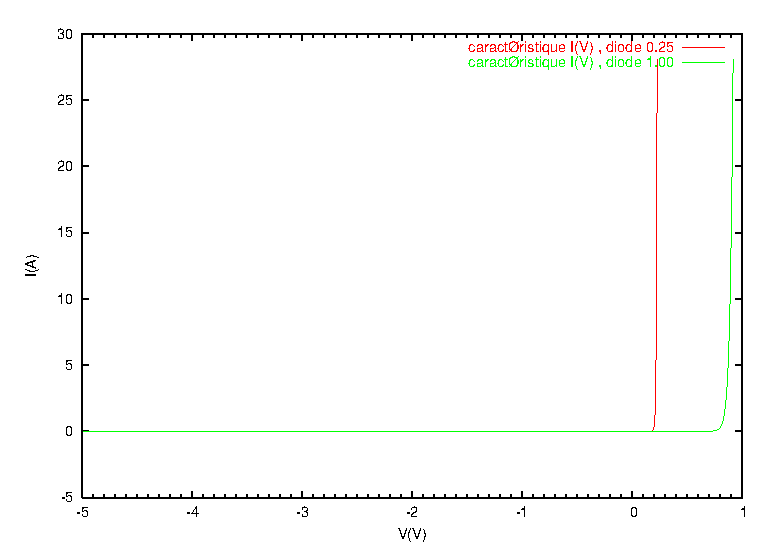
\includegraphics[width=12cm]{caracdiode.eps}
\end{center}
\caption{Diodes characteristics from SPICE model with $N=0.25$ and $N=1$}
\label{fig-carac-diode}
\end{figure}
 
The stiff diode is close to an ideal one with a threshold of $0.2$ V.

\subsection{Simulation results}
Figure (\ref{fig-comp-SMASH-SICONOS-TRAP1us}) displays a comparison of the SMASH and SICONOS results with
a trapezoidal integration ($\theta = 0.5$) and a fixed time step of 1 $\mu$s. A stiff diode model was used in SMASH simulations.
One can notice that the results from both simulators are very close. The slight differences are due to the smooth 
model of the diode used by SMASH, and mainly to the threshold of around 0.2 V. Such a threshold
yields small differences in the conduction state of the diode with respect to the ideal diode.

\begin{figure}[hbt]
\begin{center}
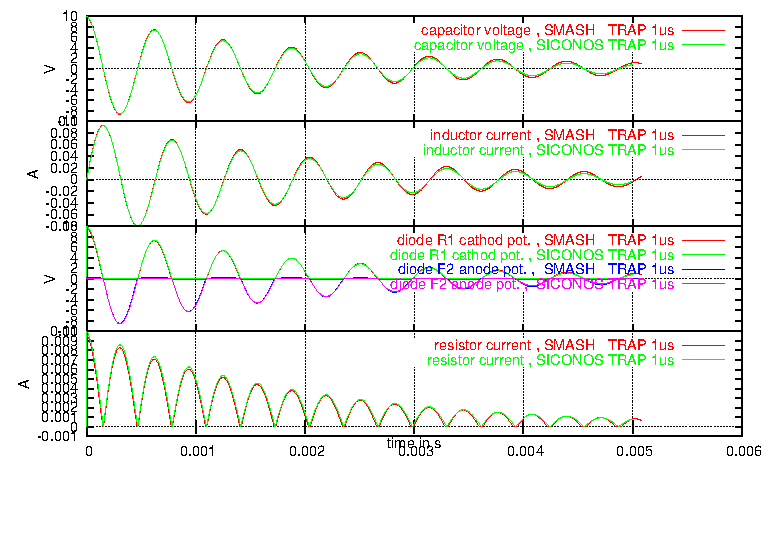
\includegraphics[width=12cm]{comp_SMASH_SICONOS_TRAP1us.eps}
\end{center}
\caption{SMASH and SICONOS simulation results with trapezoidal integration, 1 $\mu$s time step}
\label{fig-comp-SMASH-SICONOS-TRAP1us}
\end{figure}


\end{document}
